\documentclass[border=10pt]{standalone}

\usepackage{tikz}
\usepackage{tikzsymbols}
\usetikzlibrary{calc,patterns,shapes.geometric}

\def\centerarc[#1](#2)(#3:#4:#5){\draw[#1] ($(#2)+({#5*cos(#3)},{#5*sin(#3)})$) arc (#3:#4:#5);}

\begin{document}
	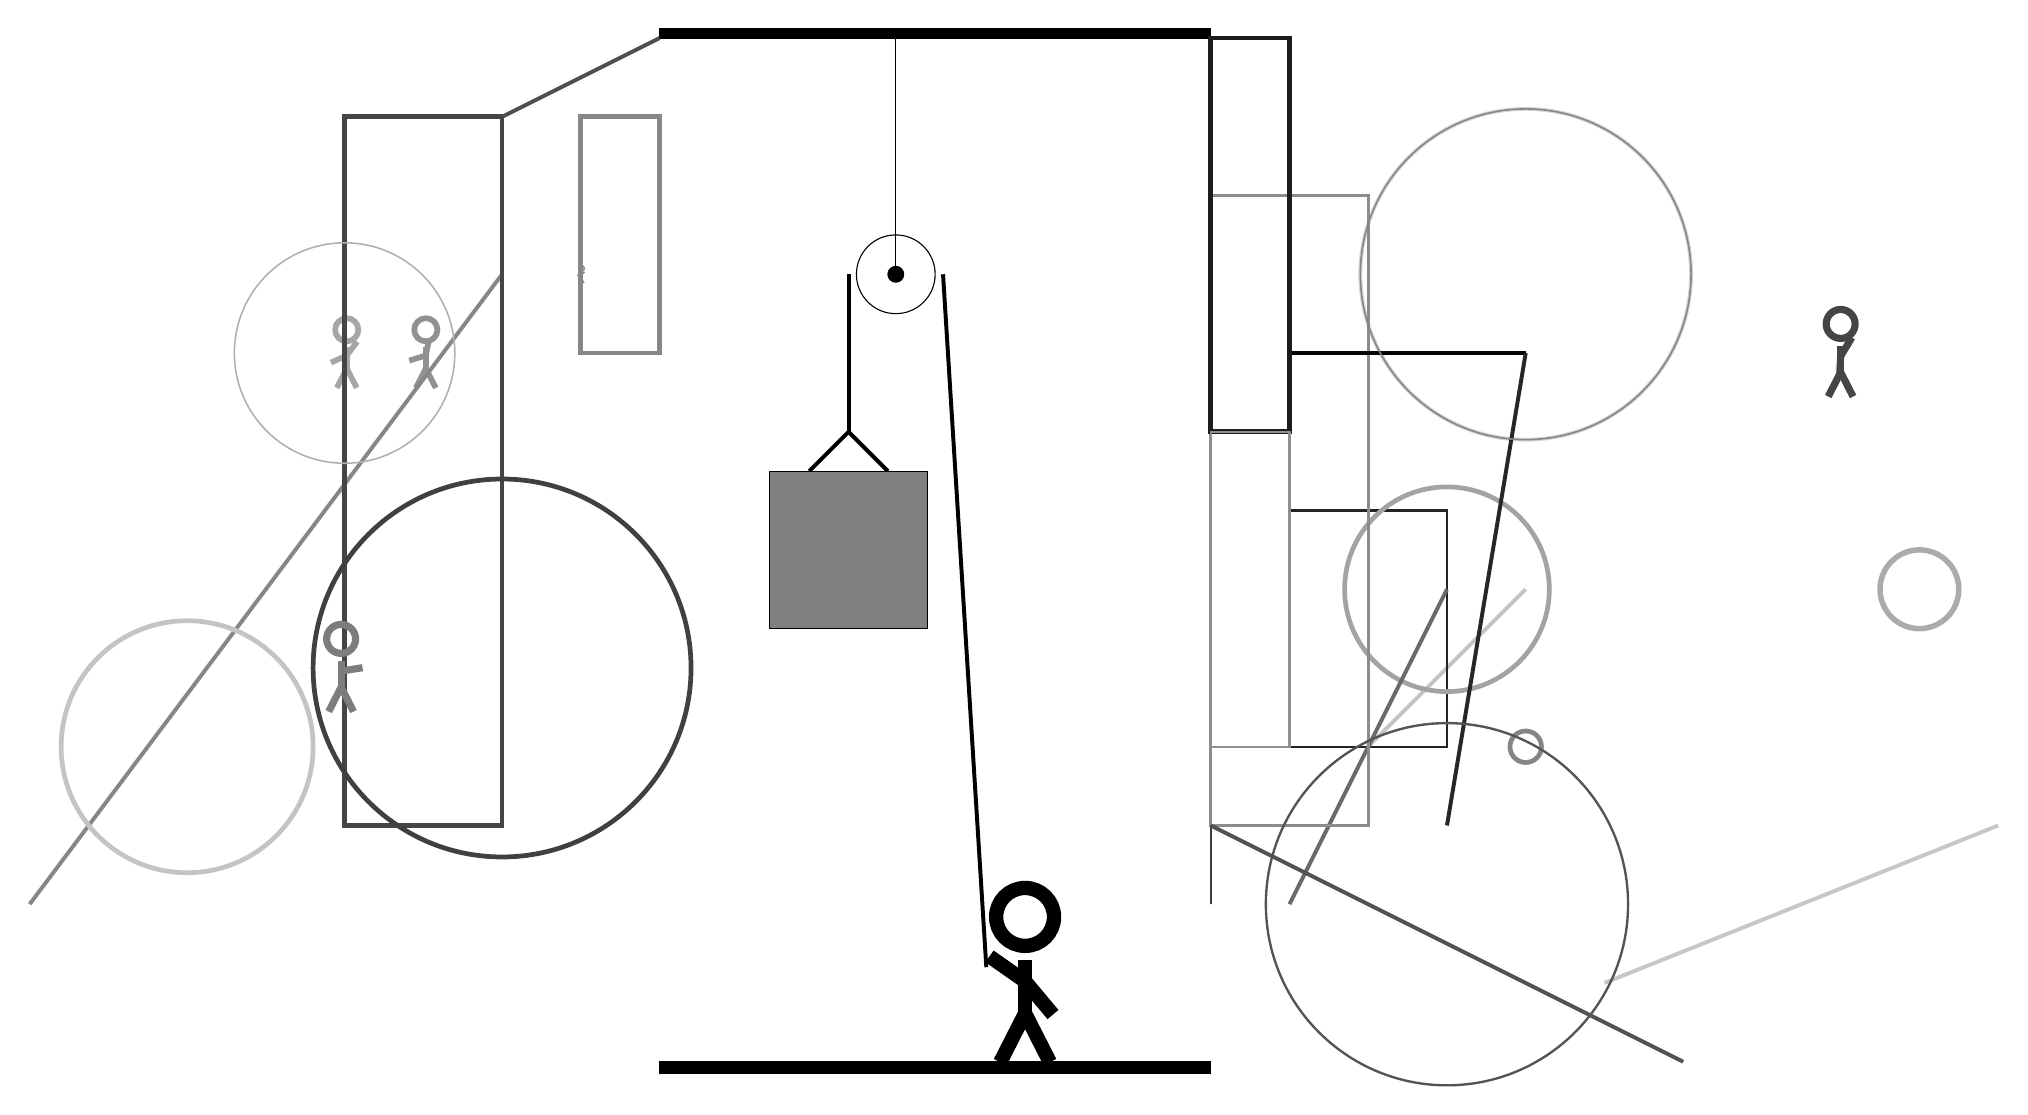
\begin{tikzpicture}
		%%%%% START %%%%%
		
		\draw[fill=black] (-2, 10) rectangle (5, 10.125);
		
		\draw (1, 7) circle (0.5);
		\draw[fill=black] (1, 7) circle (0.1);
		\draw (1, 10) -- (1, 7);
		
		\node[line width=0.2mm, color=black!43] at (-5, 6) {\Strichmaxerl[4][17][79]};
		
		\draw[line width=0.5mm, color=black!23](7, 1) -- (9, 3);
		\draw[line width=0.3mm, color=black!86] (6, 1) rectangle (8, 4);
		\draw[line width=0.3mm, color=black!60] (-4, 2) rectangle (-4, 0);
		\draw [line width=0.6mm, color=black!36](8, 3) circle (1.3);
		
		\draw[line width=0.5mm, color=black!59](8, 3) -- (6, -1);
		\draw[line width=0.5mm, color=black!47](-4, 7) -- (-10, -1);
		\draw [line width=0.5mm, color=black!16](9, 7) circle (2.1);
		\node[line width=0.3mm, color=black!47] at (-3, 7) {\Strichmaxerl[1][6][46]};
		
		\draw[line width=0.4mm, color=black!45] (5, 8) rectangle (7, 0);
		
		\draw[line width=0.3mm, color=black!77] (5, -1) rectangle (5, 0);
		\node[line width=0.5mm, color=black!35] at (-6, 6) {\Strichmaxerl[4][24][53]};
		\draw [line width=0.2mm, color=black!31](-5, 2) circle (0.0);
		
		\draw[line width=0.6mm, color=black!73] (-4, 0) rectangle (-6, 9);
		\draw[line width=0.6mm, color=black!47] (-3, 6) rectangle (-2, 9);
		\draw[line width=0.5mm, color=black!99](9, 6) -- (6, 6);
		\draw [line width=0.7mm, color=black!33](14, 3) circle (0.5);
		\draw[line width=0.5mm, color=black!69](-2, 10) -- (-4, 9);
		\draw[line width=0.5mm, color=black!22](10, -2) -- (15, 0);
		
		\node[line width=0.3mm, color=black!73] at (13, 6) {\Strichmaxerl[5][87][59]};
		\draw [line width=0.6mm, color=black!75](-4, 2) circle (2.4);
		\draw [line width=0.6mm, color=black!23](-8, 1) circle (1.6);
		\draw [line width=0.6mm, color=black!48](9, 1) circle (0.2);
		\draw[line width=0.5mm, color=black!85](8, 0) -- (9, 6);
		\draw [line width=0.2mm, color=black!31](-6, 6) circle (1.4);
		
		\draw [line width=0.2mm, color=black!48](9, 7) circle (2.1);
		
		\draw[line width=0.6mm, color=black!89] (5, 5) rectangle (6, 10);
		\draw[line width=0.5mm, color=black!68](5, 0) -- (11, -3);
		
		\draw [line width=0.3mm, color=black!67](8, -1) circle (2.3);
		
		\node[line width=0.2mm, color=black!51] at (-6, 2) {\Strichmaxerl[5][90][9]};
		\draw[line width=0.3mm, color=black!44] (6, 1) rectangle (5, 5);
		
		
		\draw[line width=0.5mm] (-0.1, 4.5) -- (0.4, 5.0) -- (0.9, 4.5);
		\draw[fill=black!50] (-0.6, 4.5) rectangle (1.4, 2.5);
		
		\draw[line width=0.5mm] (0.4, 7) -- (0.4, 5.0);
		\centerarc[line width=0.5mm](1, 7)(0:180:0.6);
		\draw[line width=0.5mm](1.6, 7) -- (2.15, -1.8);
		
		\node at (2.6, -1.9) {\Strichmaxerl[10][-35][-50]};
		
		\draw[fill=black] (-2, -3) rectangle (5, -3.15);
		
		%%%%% END %%%%%
	\end{tikzpicture}
\end{document}